% Options for packages loaded elsewhere
\PassOptionsToPackage{unicode}{hyperref}
\PassOptionsToPackage{hyphens}{url}
\PassOptionsToPackage{dvipsnames,svgnames*,x11names*}{xcolor}
%
\documentclass[
]{article}
\usepackage{lmodern}
\usepackage{amssymb,amsmath}
\usepackage{ifxetex,ifluatex}
\ifnum 0\ifxetex 1\fi\ifluatex 1\fi=0 % if pdftex
  \usepackage[T1]{fontenc}
  \usepackage[utf8]{inputenc}
  \usepackage{textcomp} % provide euro and other symbols
\else % if luatex or xetex
  \usepackage{unicode-math}
  \defaultfontfeatures{Scale=MatchLowercase}
  \defaultfontfeatures[\rmfamily]{Ligatures=TeX,Scale=1}
\fi
% Use upquote if available, for straight quotes in verbatim environments
\IfFileExists{upquote.sty}{\usepackage{upquote}}{}
\IfFileExists{microtype.sty}{% use microtype if available
  \usepackage[]{microtype}
  \UseMicrotypeSet[protrusion]{basicmath} % disable protrusion for tt fonts
}{}
\makeatletter
\@ifundefined{KOMAClassName}{% if non-KOMA class
  \IfFileExists{parskip.sty}{%
    \usepackage{parskip}
  }{% else
    \setlength{\parindent}{0pt}
    \setlength{\parskip}{6pt plus 2pt minus 1pt}}
}{% if KOMA class
  \KOMAoptions{parskip=half}}
\makeatother
\usepackage{xcolor}
\IfFileExists{xurl.sty}{\usepackage{xurl}}{} % add URL line breaks if available
\IfFileExists{bookmark.sty}{\usepackage{bookmark}}{\usepackage{hyperref}}
\hypersetup{
  pdftitle={"Population PK-QT Analysis Example"},
  pdfauthor={Ana Ruiz-Garcia, PharmD, PhD, Metrum Research Group Steve Riley, PharmD, PhD, Pfizer Inc Dhananjay Marathe, PhD, Merck \& Co Inc},
  colorlinks=true,
  linkcolor=blue,
  filecolor=Maroon,
  citecolor=Blue,
  urlcolor=Blue,
  pdfcreator={LaTeX via pandoc}}
\urlstyle{same} % disable monospaced font for URLs
\usepackage[left=3.5cm,right=3.5cm,top=3cm,bottom=3cm]{geometry}
\usepackage{graphicx,grffile}
\makeatletter
\def\maxwidth{\ifdim\Gin@nat@width>\linewidth\linewidth\else\Gin@nat@width\fi}
\def\maxheight{\ifdim\Gin@nat@height>\textheight\textheight\else\Gin@nat@height\fi}
\makeatother
% Scale images if necessary, so that they will not overflow the page
% margins by default, and it is still possible to overwrite the defaults
% using explicit options in \includegraphics[width, height, ...]{}
\setkeys{Gin}{width=\maxwidth,height=\maxheight,keepaspectratio}
% Set default figure placement to htbp
\makeatletter
\def\fps@figure{htbp}
\makeatother
\setlength{\emergencystretch}{3em} % prevent overfull lines
\providecommand{\tightlist}{%
  \setlength{\itemsep}{0pt}\setlength{\parskip}{0pt}}
\setcounter{secnumdepth}{5}
\usepackage{float}
\usepackage{longtable}
\usepackage{caption}
\usepackage{titling}
\usepackage{booktabs}
\pretitle{\begin{center} 
\includegraphics[width=2in,height=2in]{logo.jpg}\LARGE\\}
\posttitle{\end{center}}
\usepackage[T1]{fontenc}
\usepackage[utopia]{mathdesign}
\usepackage[]{natbib}
\bibliographystyle{plainnat}

\title{\vspace{8cm}\LARGE"Population PK-QT Analysis Example"\vspace{4cm}}
\author{Ana Ruiz-Garcia, PharmD, PhD, Metrum Research Group\\
Steve Riley, PharmD, PhD, Pfizer Inc\\
Dhananjay Marathe, PhD, Merck \& Co Inc}
\date{``September 09, 2020''}

\begin{document}
\maketitle

\centering

\raggedright

\clearpage

\tableofcontents

\newpage

\hypertarget{introduction}{%
\section{Introduction}\label{introduction}}

The International Council for Harmonization (ICH) revised the
\href{https://database.ich.org/sites/default/files/E14_Q\%26As_R3_Q\%26As.pdf}{E14
Q\&A (R3)} allowing a population PK-QT modeling to be used as primary
analysis for assessing the QTc interval prolongation risk of new drug
entities.

PK-QT analysis is intended to determine whether the studied drug has a
threshold pharmacologic effect on cardiac repolarization, as detected by
QTc prolongation.

\hypertarget{objectives}{%
\section{Objectives}\label{objectives}}

\begin{itemize}
\tightlist
\item
  To perform a population PK-QT analysis to characterize the
  exposure-response (E-R) relationship between moxifloxacin and the risk
  of cardiac repolarization, detected by QTc prolongation
\end{itemize}

\hypertarget{data-sources-and-description}{%
\section{Data Sources and
Description}\label{data-sources-and-description}}

Moxifloxacin data were extracted from the
\href{https://pubmed.ncbi.nlm.nih.gov/25670536/}{IQ-CSRC study} wherein
5 QT-prolonging drugs and 1 drug for which no QT prolongation was
observed in a through QT (TQT) study were evaluated to demonstrate that
E-R analysis could detect QT prolongation in small studies with healthy
volunteers.

The data we will use today are from subjects administered moxifloxacin
400 mg orally (therapeutic dose) on Day 1 followed by 800 mg IV
(supratherapeutic dose) on Day 2.

Study subjects were wearing a Holter monitor for electrocardiogram (ECG)
recording for 24 hrs. Ten ECG recordings and blood samples for PK
analysis were collected at each time point. All study treatments had
identical sample collection time points. Placebo PK samples were only to
be analyzed if deemed necessary.

Pharmacokinetic sampling and ECG assessments for placebo and
moxifloxacin were done at predose, 0.5, 1, 2, 3, 4, 6, 8, 12 and 24 hr
post-dose. Pre-dose ECG assessments were done at -30, -20, -10, and
right before dosing. Baseline ECG values were determined by the mean of
the average of the 10 recordings collected at the scheduled times. Blood
samples were taken after completion of ECG recordings.

\hypertarget{ecg-acquisition-and-measurements}{%
\subsection{ECG Acquisition and
Measurements}\label{ecg-acquisition-and-measurements}}

Describe ECG collection methodology for your study here, e.g., manually
overread at a core ECG lab, readers were/were not blinded to treatment,
each subject's ECGs were read by the same reader to minimize
between-rater variability, etc.

\hypertarget{data-manipulation}{%
\subsection{Data manipulation}\label{data-manipulation}}

Data were to be excluded if the paired ECG and PK samples were not
collected within 15 min of one another and/or if ECG or PK data were
missing for a particular time point (with the exception of baseline
assessments and placebo treatment where PK is not collected or is zero).

\hypertarget{analysis-methods}{%
\section{Analysis Methods}\label{analysis-methods}}

\hypertarget{computational-software}{%
\subsection{Computational Software}\label{computational-software}}

The population PK-QT analysis was conducted using a population approach
and linear mixed effects models. Estimation was conducted using R Studio
using R version 4.0.0 (2020-04-24) (R Foundation for Statistical
Computing, Vienna, Austria) \citep{Team2014} with the nlme package
\citep{bib:nlme} and maximum likelihood estimation or restricted maximum
likelihood estimation. Data manipulation, post-processing, and graphics
were conducted using R.

\hypertarget{model-strategy}{%
\subsection{\texorpdfstring{Model Strategy
\label{sec:strategy}}{Model Strategy }}\label{model-strategy}}

Prior to starting modeling efforts, graphical and tabular summaries were
created to check some basic assumptions that will drive the model
development:

\begin{itemize}
\item
  Drug effect on HR: The potential of the drug to significantly increase
  or decrease HR. There is no clear consensus on the specific threshold
  effect on HR that could influence QTc assessment, however, mean
  increases or decreases of greater than 10 bpm have been considered
  problematic \citep{Garnett2012-kw}
\item
  Demonstration of QT Correction: QTc interval is independent of HR for
  drug-free and/or placebo treatments. QTcF is usually sufficient
  correction method for drugs with insignificant effects on HR.
\item
  Assessment of Time Delay Between Drug Concentration and \(\Delta\)QTc:
  The default model assumption is a direct temporal relationship between
  drug concentration and QTc effect.
\end{itemize}

Following the basic model independent check the next steps are:

\begin{itemize}
\item
  Model Development
\item
  Model adequacy
\end{itemize}

\hypertarget{effect-of-moxifloxacin-on-heart-rate}{%
\subsection{Effect of Moxifloxacin on Heart
Rate}\label{effect-of-moxifloxacin-on-heart-rate}}

Prior to determining the most appropriate QT correction factor, the
effect of studied drug treatment on heart rate (HR) was evaluated to
support the assumption that the QT-HR relationship is the same
regardless of the presence or absence of drug. Plots were generated of
the mean change from baseline HR versus time grouped by treatment.

A linear mixed-effect model (LME) was used to evaluate the linear
relationship between HR and moxifloxacin concentration.

\begin{equation} \label{HReq}
\Delta HR_{ijk}=(\theta_j + \beta_{0k} + \eta_{0,i})+\gamma \times(HR_{ij0}-\overline{HR}_{ij0})+(\beta_1 +\eta_{1,i}) \times C_{ijk} +\epsilon_{ijk}
\end{equation}

where \(\Delta HR_{ijk}\) is the change from baseline HR for the
i\(^{th}\) subject, in the j\(^{th}\) treatment, at the k\(^{th}\) time
point (nominal) relative to dosing;j=1 for active drug (moxifloxacin)
and j=0 for placebo; \(C_{ijk}\) is the concentration at the k\(^{th}\)
time point for the j\(^{th}\) treatment in the i\(^{th}\)
subject(\(C_{ijk}\)=0 for placebo); \(\theta_j\) is the
treatment-specific intercept (moxifloxacin versus placebo),
\(\beta_{0k}\) is the population mean \(\Delta\)HR (change from
baseline) with placebo for time k (representing categorical fixed effect
of time to account for diurnal variation); \(HR_{ij0}\) is the baseline
HR for the i\(^{th}\) subject in the j\(^{th}\) treatment,
\(\overline{HR}_{ij0}\) is the overall population mean of all baseline
HR (\(HR_{ij0}\)) values (from combined placebo and active treatment
periods), and \(\gamma\) is the influence of the baseline HR (centered
on population baseline). \(\beta_1\) is the slope which quantifies the
relationship between \(\Delta\) HR and concentration. \(\eta_{0,i}\) and
\(\eta_{1,i}\) are the subject-specific random effects (inter-individual
variability) for the intercept and slope, respectively, each with a mean
of zero and variance \(\omega^2\), and \(\epsilon_{ijk}\) is the
residual error of the i\(^{th}\) subject on the j\(^{th}\) treatment at
the k\(^{th}\) time point with a mean of zero and variance \(\sigma^2\).

\hypertarget{demonstration-of-qt-correction}{%
\subsection{Demonstration of QT
Correction}\label{demonstration-of-qt-correction}}

The preferred QT correction (unless the studied drug has a significant
effect on HR) is the Fridericia heart-rate corrected QT interval (QTcF).
Unless drug-free QT data is collected in all subjects over a range of
heart rates similar to the range of heart rates observed during
treatment, the use of subject- and study-specific corrections is not
generally recommended.

If studied drug was determined to have no effect on HR (or RR), then a
fixed correction was applied to remove the underlying HR effect on the
QT interval. The QTcF was the primary correction method in this
analysis; if data suggested this method did not adequately correct for
the relationship between HR and QT interval, a more appropriate
correction could be estimated and reported.

For fixed corrections, QT interval corrected for heart rate equation is
decribed below: \begin{equation} \label{QTcor}
QTc=\frac{QT_{i,j}}{\left(\frac{RR_{i,j}}{1000} \right)^\beta}
\end{equation}

where i represents the i\(^{th}\) individual and j represents the
j\(^{th}\) measurement time for QT and RR (presented in milliseconds).
The subject- and population-specific correction factor for calculation
of QTcS could be estimated by fitting a LME model to only baseline
(pre-dose values on Day 1) individual singlets (not the averaged
triplicate) QT and RR measurements from all four study treatment periods
as described in equation \ref{QTcorind}:

\begin{equation} \label{QTcorind}
ln(QT_{i,j}) = (\theta_1 + \eta_{1,i}) + (\theta_2 + \eta_{2,i}) \cdot ln(RR_{i,j}) + \epsilon_{i,j}
\end{equation}

where ln designates natural logarithmically transformed parameter, i
represents the i\(^{th}\) individual and j represents the j\(^{th}\)
measurement time for QT (milliseconds) and RR (seconds), \(\theta_2\)
represent the study population specific estimate of the correction
factor (\(\beta\)), and \(\theta_1\) is the intercept. \(\eta_{1,i}\)
and \(\eta_{2,i}\) are the subject-specific random effects
(inter-individual variability) for the intercept and slope,
respectively, each with a mean of zero and variance \(\omega^2\), and
\(\epsilon\) is the residual error with a mean of zero and variance
\(\sigma^2\).

Thus, \(\theta_2\) and \(\theta_2\) + \(\eta_{2,i}\) represent the
study- and subject-specific estimates of the correction factor
(\(\beta\)), respectively.

The analysis dataset used in this workshop is insufficient for an
appropriate estimation of individual- and/or study-specific corrections.
Therefore, plots of QT, QTcF, and QTcB versus RR interval were generated
using only baseline singlet data to assess the adequacy of each
correction factor, to ensure that the correlation between QT and RR was
adequately removed with the correction. Comparison of correction methods
was made on the basis of the slope estimates from a LME model of QTc as
a function of RR as follows:

\begin{equation} \label{QTlme}
QTc_{i,j} = (\theta_{int} + \eta_{int,i}) + (\theta_{slope} + \eta_{slope,i}) \cdot RR_{i,j} + \epsilon_{i,j}
\end{equation}

Where QTc is the dependent variable (either QTcF, QTcB), i represents
the i\(^{th}\) individual and j represents the j\(^{th}\) measurement
time for QTc and RR, \(\theta_{int}\) is the intercept, and
\(\theta_{slope}\) quantifies the relationship between QTc and RR.
\(\eta_{int,i}\) and \(\eta_{slope,i}\) are the subject-specific random
effects (inter-individual variability) for the intercept and slope,
respectively, each with a mean of zero and variance \(\omega^2\), and
\(\epsilon\) is the residual error with a mean of zero and variance
\(\sigma^2\).

The QTc associated with the regression that generated the smallest
absolute value of the slope estimate was deemed the most appropriate HR
adjusted QT method for use as the dependent variable in the subsequent
E-R modeling; ideally the 95\% CI for the slope should contain zero.

\hypertarget{assessment-of-time-delay-between-drug-concentration-and-deltaqtc}{%
\subsection{\texorpdfstring{Assessment of Time Delay Between Drug
Concentration and
\(\Delta\)QTc}{Assessment of Time Delay Between Drug Concentration and \textbackslash DeltaQTc}}\label{assessment-of-time-delay-between-drug-concentration-and-deltaqtc}}

Concordance, or lack thereof, in the time course of studied drug
concentrations and QTcF was evaluated by:

\begin{itemize}
\tightlist
\item
  Examining the mean concentration and placebo-corrected change from
  baseline QTcF (\(\Delta \Delta\)QTcF) profiles by dose level.
\item
  Linear QTc-drug concentration relationship: a QTc\_drug concentration
  plot incorporating a trend line (i.e, loess or linear regression). The
  trend line does not reflect a model fit of data but rather is used to
  detect drug effect and linear assumption. If no delay between peak
  studied drug concentration and peak QTc effect (hysteresis) is
  apparent as assessed by visual inspection then a direct temporal
  relationship can be supported.
\end{itemize}

\hypertarget{characterization-of-moxifloxacin-exposure-response-relationship-for-qtc}{%
\subsection{\texorpdfstring{Characterization of Moxifloxacin
Exposure-Response Relationship for QTc
\label{sec:modelfit}}{Characterization of Moxifloxacin Exposure-Response Relationship for QTc }}\label{characterization-of-moxifloxacin-exposure-response-relationship-for-qtc}}

Once the basic assumptions described in Section \ref{sec:strategy} were
satisfied, then the relationship was evaluated with the pre-specified
LME model shown below. In this model the change from baseline QTcF
(\(\Delta\)QTcF) and concentration data from both placebo and
moxifloxacin treatment periods (therapeutic and supratherapeutic doses)
were analyzed. This base model to describe the dependent variable,
\(\Delta\)QTc, includes the following fixed effect parameters:
intercept, slope, the effect of treatment (categorical), time
(categorical), and baseline QTc (continuous) on the intercept.
Characterizing the placebo response at each nominal time point accounts
for the effect of diurnal variation in QTc. Subject is included as a
random effect on both the intercept and slope.

\begin{equation} \label{E-R}
\Delta QTc_{ijk} = (\theta_j + \beta_{0k} + \eta_{0,i}) + \gamma \cdot (QTc_{ij0} - \overline{QTc}_{ij0}) + (\beta_1 + \eta_{1,i}) \cdot C_{ijk} + \epsilon_{ijk}
\end{equation}

where \(\Delta\) \(QTc_{ijk}\) is the change from baseline QTc interval
for the i\(^{th}\) subject, in the j\(^{th}\) treatment, at the
k\(^{th}\) time point (nominal) relative to dosing; j=1 for active drug
(moxifloxacin) and j=0 for placebo; \(\theta_j\) is the
treatment-specific intercept (moxifloxacin versus placebo),
\(\beta_{0k}\) is the population mean \(\Delta\)QTc (change from
baseline) in the placebo group at each time k (representing categorical
fixed effect of time to account for diurnal variation); \(\gamma\) is
the influence of the baseline QTc (centered on population baseline);
\(QTc_{ij0}\) is the baseline QTc for the i\(^{th}\) subject in the the
j\(^{th}\) treatment, \(\overline{QTc}_{ij0}\) is the overall population
mean of all baseline QTc (\(QTc_{ij0}\)) values (from combined placebo
and active treatment periods), and \(C_{ijk}\) is the concentration in
the i\(^{th}\) subject (and \(C_{i0k}\)=0 for placebo) for the
j\(^{th}\) treatment at the k\(^{th}\) time point; \(\beta_1\) is the
slope which quantifies the relationship between \(\Delta\)QTc and
concentration. \(\eta_{0,i}\) and \(\eta_{1,i}\) are the
subject-specific random effects (inter-individual variability) for the
intercept and slope, respectively, each with a mean of zero and variance
\(\omega^2\), and \(\epsilon_{ijk}\) is the residual error of the
i\(^{th}\) subject on the j\(^{th}\) treatment at the k\(^{th}\) time
point with a mean of zero and variance \(\sigma^2\).

The \(\Delta\)QTc versus concentration model was used to compute the
placebo-adjusted change from baseline QTc (\(\Delta\Delta\)QTc) over the
observed concentration range. The model-derived \(\Delta\Delta\)QTc is
the difference between the model-derived \(\Delta\)QTc at a given
concentration under moxifloxacin treatment, and the model-derived
\(\Delta\)QTc under placebo treatment with drug concentration equal to
zero. Using the contrast function (contrast package)
\citep{bib:contrast} in R and the \(\Delta\)QTc model object, the mean
and two-sided 90\% CI for the predicted population average
\(\Delta\Delta\)QTc at concentrations of interest (Cmax) can be computed
as follows in Equations \ref{QTeq} and \ref{CI90}.

\begin{equation} \label{QTeq}
mean \Delta \Delta \overline{QTc}(C) = mean (\Delta \overline{QTc}_{ijk}|j= 1;C_{ijk} =C)-mean (\Delta \overline{QTc}_{ijk}|j = 0;C_{ijk} = 0) 
\end{equation}

where \emph{mean}\(\Delta\Delta\overline{QTc}_{ijk}\)\textbar{} \emph{j}
= 1;\(C_{ijk}\) = C is the predicted population average \(\Delta\)QTc
under moxifloxacin treatment at plasma concentration C, and
\emph{mean}\(\Delta QTc_{ijk}\)\textbar{} \emph{j} = 0;\(C_{ijk}\) is
the predicted population average \(\Delta\)QTc in the absence of drug
(i.e.~placebo treatment where C = 0).

\begin{equation} \label{CI90}
90\% CI = mean \Delta \Delta \overline{QTc}(C) \pm t(0.90, DF) \cdot SE (mean \Delta \Delta \overline{QTc}(C)) 
\end{equation}

where t is the critical value determined from the t-distribution, DF is
the degrees of freedom, and SE is the standard error.

\hypertarget{model-adequacy}{%
\subsection{Model Adequacy}\label{model-adequacy}}

The evaluation of the model fit was based on several goodness-of-fit
(GOFs) plots:

\begin{itemize}
\tightlist
\item
  Scatter plots of model predicted (population and individual) versus
  observed \(\Delta\)QTc values with line of unity and loess line, to
  demonstrate any patterns suggestive of concentration dependent
  over/under prediction of \(\Delta\)QTc
\item
  Scatter plots of population and individual standardized (Pearson
  weighted) residuals versus \(\Delta\)QTc and drug concentration,
\item
  Boxplots of standardized residuals versus nominal time post dose and
  treatment (categorical variables) and quantile-quantile (Q-Q) plots of
  the standardized residuals to check that residuals follow normal
  distribution with mean of zero
\item
  Scatter and quantile plots of concentration were used for displaying
  mean baseline corrected QTc (\(\Delta\)QTc) and associated 90\% CI
  derived from the observed data, with model predicted variables and the
  associated 90\% CI overlayed. Systematic differences between the model
  predictions and observed data would suggest model misspecification
\end{itemize}

\hypertarget{results}{%
\section{Results}\label{results}}

A total of 13 subjects were enrolled, 6 subjects were administered with
placebo and 9 subjects were administered with 2 doses of moxifloxacin.
Out of the subjects administered with placebo, 2 received moxifloxacin.
Time-matched ECG collections from the placebo treatment group were used
to correct for diurnal patterns in QTc data.

The time course of the mean (\(\pm\)SD) change from baseline QTcF
intervals by treatment is displayed in Figure
\ref{fig:DQTCFbytreatment}.

\begin{figure}[H]
\caption{Mean QTcF Change From Baseline Over Time by Treatment Group} 
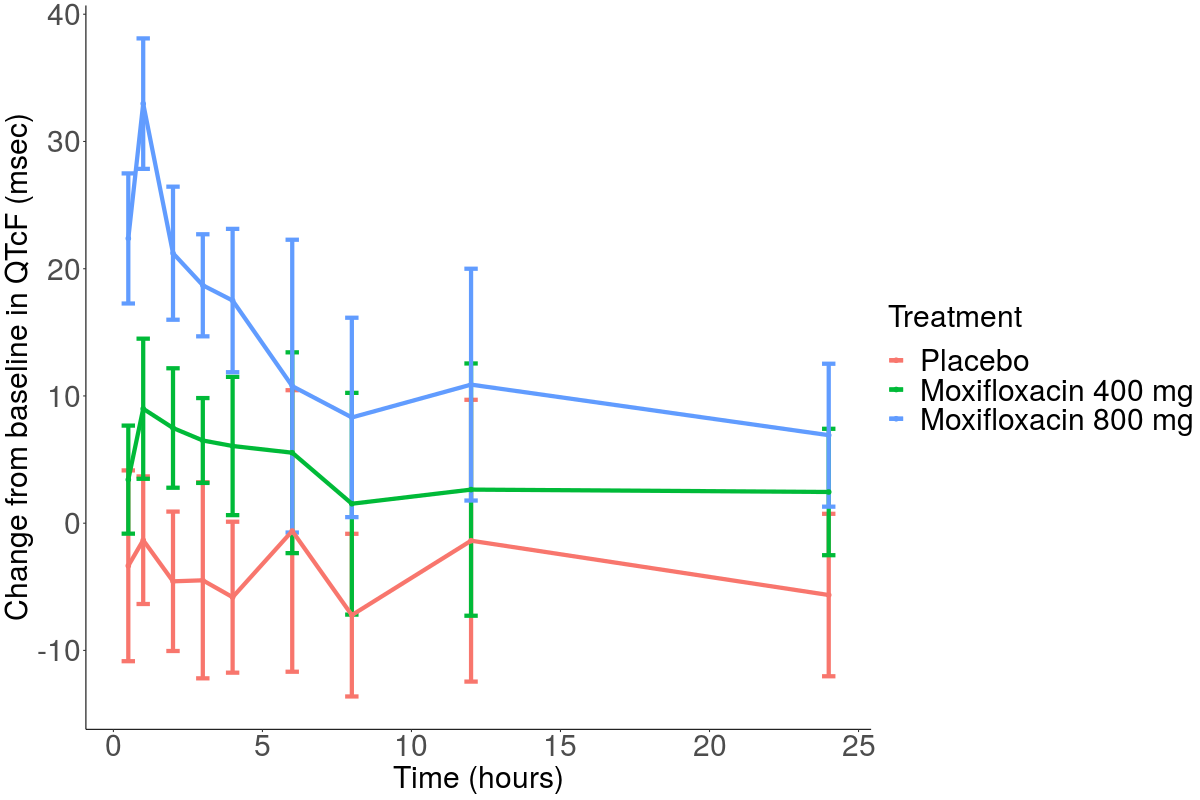
\includegraphics[width=\textwidth]{../Report/Figures/DQTCFbytreatment.png}
\label{fig:DQTCFbytreatment}
\end{figure}

Tables \ref{tab:delta_placebosum} and \ref{tab:delta_moxisum} display
summary statistics for \(\Delta\)QTcF intervals by timepoint for the
placebo group and the 2 doses of moxifloxacin, respectively.

\clearpage

\captionsetup{justification = RaggedRight,singlelinecheck=false}
\captionof{table}{Summary of Baseline-Corrected ($\Delta$QTcF) Intervals For the Placebo Treatment per Timepoint}

\begin{tabular}{rrrll}
\toprule
Day & Nominal Time (hrs) & N & Mean (SD) & Median (Max, Min)\\
\midrule
1 & 0.5 & 6 & -3.23 ( 6.82 ) & -3.52 ( 5.13 , -13.18 )\\
1 & 1.0 & 6 & -2.45 ( 5.37 ) & -2.81 ( 4.01 , -9.27 )\\
1 & 2.0 & 6 & -4.01 ( 6.09 ) & -5.01 ( 4.91 , -13.43 )\\
1 & 3.0 & 6 & -3.83 ( 4.37 ) & -4.91 ( 3.61 , -7.86 )\\
1 & 4.0 & 6 & -4.63 ( 5.75 ) & -6.86 ( 5.15 , -9.93 )\\
1 & 6.0 & 6 & 1.68 ( 11.09 ) & 1.64 ( 16.11 , -10.05 )\\
1 & 8.0 & 6 & -4.96 ( 5.88 ) & -6.79 ( 4.21 , -10.3 )\\
1 & 12.0 & 6 & -1.02 ( 12.24 ) & -1.66 ( 18.15 , -16.07 )\\
1 & 24.0 & 6 & -4.67 ( 4.86 ) & -6.13 ( 1.82 , -10.89 )\\
2 & 0.5 & 6 & -3.46 ( 8.79 ) & -5.96 ( 13.33 , -10.05 )\\
2 & 1.0 & 6 & -0.22 ( 4.85 ) & -1.78 ( 9.13 , -3.95 )\\
2 & 2.0 & 6 & -5.13 ( 5.31 ) & -5.82 ( 1.68 , -12.55 )\\
2 & 3.0 & 6 & -5.16 ( 10.51 ) & -9.04 ( 13.27 , -14.05 )\\
2 & 4.0 & 6 & -7 ( 6.41 ) & -8.81 ( 5.41 , -12.27 )\\
2 & 6.0 & 6 & -2.91 ( 11.57 ) & -3.96 ( 14.71 , -14.67 )\\
2 & 8.0 & 6 & -9.49 ( 6.56 ) & -11.69 ( 0.91 , -15.65 )\\
2 & 12.0 & 6 & -1.73 ( 10.94 ) & -1.52 ( 9.82 , -15.07 )\\
2 & 24.0 & 6 & -6.63 ( 7.99 ) & -8.81 ( 7.03 , -14.15 )\\
\bottomrule
\end{tabular}


\label{tab:delta_placebosum}

\clearpage

\captionsetup{justification = RaggedRight,singlelinecheck=false}
\captionof{table}{Summary of Baseline-Corrected ($\Delta$QTcF) Intervals For Moxifloxacin per Dose and Timepoint}

\begin{tabular}{rrrll}
\toprule
Day & Nominal Time (hrs) & N & Mean (SD) & Median (Max, Min)\\
\midrule
1 & 0.5 & 9 & 3.42 ( 4.25 ) & 3.81 ( 8.38 , -3.99 )\\
1 & 1.0 & 9 & 8.99 ( 5.51 ) & 10.26 ( 14.36 , -2.22 )\\
1 & 2.0 & 9 & 7.48 ( 4.69 ) & 6.81 ( 16.17 , 1.19 )\\
1 & 3.0 & 9 & 6.5 ( 3.34 ) & 7.09 ( 11.92 , 0.88 )\\
1 & 4.0 & 9 & 6.06 ( 5.43 ) & 4.89 ( 16.87 , 0.4 )\\
1 & 6.0 & 9 & 5.54 ( 7.89 ) & 3.47 ( 18.77 , -5.77 )\\
1 & 8.0 & 9 & 1.53 ( 8.71 ) & -0.65 ( 18.56 , -10.93 )\\
1 & 12.0 & 9 & 2.64 ( 9.92 ) & 4.86 ( 18.08 , -11.67 )\\
1 & 24.0 & 9 & 2.45 ( 4.97 ) & 1.91 ( 10.66 , -4.87 )\\
2 & 0.5 & 9 & 22.38 ( 5.11 ) & 23.13 ( 30.07 , 14.06 )\\
2 & 1.0 & 9 & 32.98 ( 5.13 ) & 32.22 ( 43.77 , 25.48 )\\
2 & 2.0 & 9 & 21.22 ( 5.23 ) & 19.87 ( 28.96 , 14.76 )\\
2 & 3.0 & 9 & 18.7 ( 4.01 ) & 19.71 ( 25.48 , 13.83 )\\
2 & 4.0 & 9 & 17.5 ( 5.63 ) & 14.49 ( 25.18 , 10.88 )\\
2 & 6.0 & 9 & 10.77 ( 11.5 ) & 9.66 ( 28.38 , -4.84 )\\
2 & 8.0 & 9 & 8.31 ( 7.84 ) & 7.68 ( 24.68 , -1.94 )\\
2 & 12.0 & 9 & 10.89 ( 9.11 ) & 13.98 ( 25.58 , -3.01 )\\
2 & 24.0 & 9 & 6.91 ( 5.62 ) & 6.77 ( 16.96 , -2.77 )\\
\bottomrule
\end{tabular}


\label{tab:delta_moxisum}

\clearpage

Following administration of single PO doses of moxifloxacin 400 mg and
800 mg, peak plasma moxifloxacin concentration Cmax was achieved with a
median time to maximum concentration (Tmax) of 1-3 hours post dose. The
observed geometric mean (geometric coefficient of variation (CV)\%) of
Cmax in ng/mL at the 400 mg (therapeutic) and 800 mg (supratherapeutic)
doses were 1862.14 ( 28.36 ) and 4576.13 ( 20.98 ), respectively. Mean
moxifloxacin concentration-time profiles are presented in Figure
\ref{fig:PKprofiles}. Table \ref{tab:pksum} presents summary statistics
of moxifloxacin maximum concentration per dose group.

\begin{figure}[H]
\caption{Mean Moxifloxacin Concentration-Time Profile by Dose Group} 
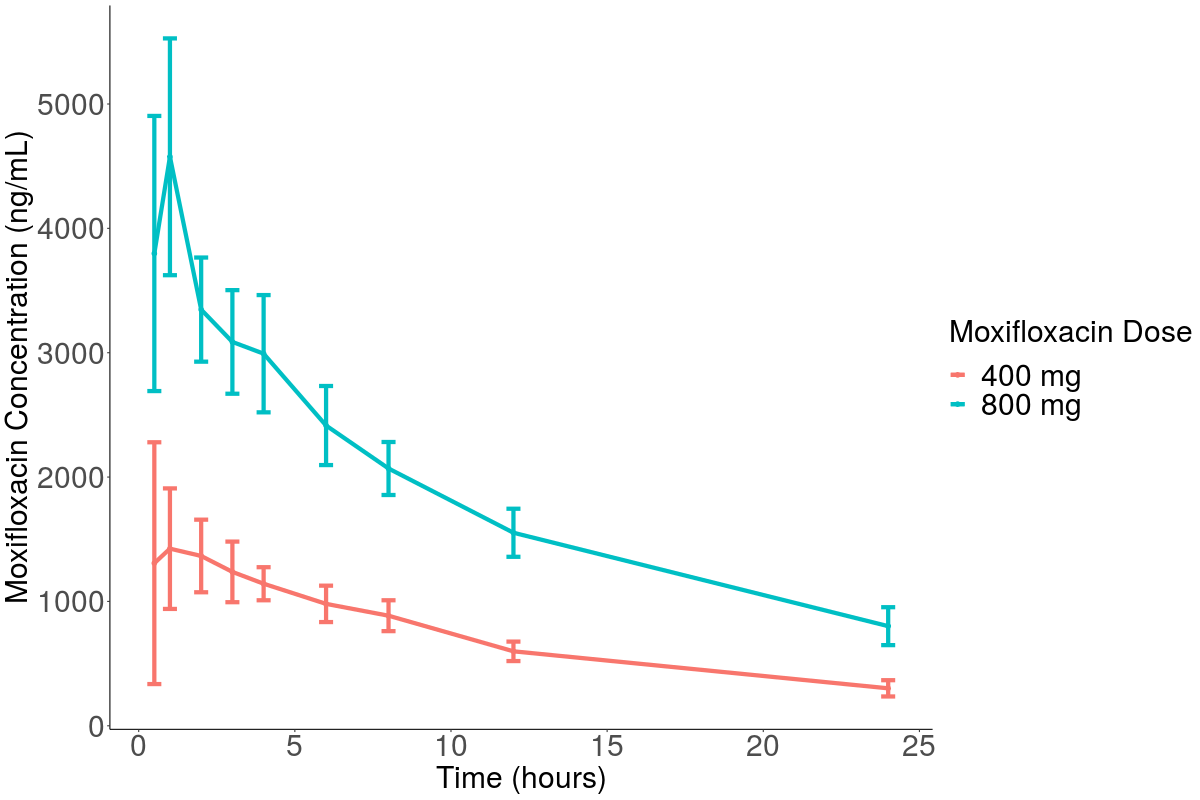
\includegraphics[width=\textwidth]{../Report/Figures/PKprofiles.png}
\label{fig:PKprofiles}
\end{figure}

\captionsetup{justification = RaggedRight,singlelinecheck=false}
\captionof{table}{Summary of Moxifloxacin Maximum Concentration by Dose}

\begin{tabular}{lll}
\toprule
Tmax Median (Max, Min) & Geometric Mean (CV\%) & Median (Max, Min)\\
\midrule
1 ( 3 , 0.5 ) & 1862.14 ( 28.36 ) & 2030 ( 3130 , 1240 )\\
1 ( 1 , 0.5 ) & 4576.13 ( 20.98 ) & 4240 ( 5800 , 3280 )\\
\bottomrule
\end{tabular}


\label{tab:pksum} \clearpage

\hypertarget{effect-of-moxifloxacin-on-heart-rate-1}{%
\subsection{Effect of Moxifloxacin on Heart
Rate}\label{effect-of-moxifloxacin-on-heart-rate-1}}

The effect of moxifloxacin on heart rate (HR) was evaluated via a linear
mixed-effects modeling with \(\Delta\)HR as the dependent variable and
moxifloxacin plasma concentration as independent variable.

\captionsetup{justification = centering}
\captionof{table}{Summary of Baseline-Corrected ($\Delta$HR)  Intervals For Moxifloxacin Treatment per Timepoint and Dose Level}

\begin{tabular}{lrrrrll}
\toprule
TRTG & DOSE & Day & Nominal Time (hrs) & N & Mean (SD) & Median (Max, Min)\\
\midrule
D - moxifloxacin & 400 & 1 & 0.5 & 9 & 2.26 ( 6.03 ) & 4.48 ( 8.63 , -8.06 )\\
D - moxifloxacin & 400 & 1 & 1.0 & 9 & 1.2 ( 5.2 ) & 0.85 ( 8.79 , -8.28 )\\
D - moxifloxacin & 400 & 1 & 2.0 & 9 & -0.55 ( 3.46 ) & -1.07 ( 4.72 , -5.01 )\\
D - moxifloxacin & 400 & 1 & 3.0 & 9 & -1.62 ( 4.14 ) & -1.47 ( 7.65 , -6.93 )\\
D - moxifloxacin & 400 & 1 & 4.0 & 9 & -0.12 ( 5.38 ) & -0.73 ( 10.45 , -6.29 )\\
D - moxifloxacin & 400 & 1 & 6.0 & 9 & 9.48 ( 6.23 ) & 10.41 ( 17.13 , -0.23 )\\
D - moxifloxacin & 400 & 1 & 8.0 & 9 & 6.16 ( 5.47 ) & 4.11 ( 15.03 , -2.51 )\\
D - moxifloxacin & 400 & 1 & 12.0 & 9 & 11.22 ( 7.31 ) & 12.69 ( 22.43 , -1.03 )\\
D - moxifloxacin & 400 & 1 & 24.0 & 9 & 0.65 ( 5.93 ) & -1.37 ( 10.11 , -8.93 )\\
D - moxifloxacin & 800 & 2 & 0.5 & 9 & 4.98 ( 7.8 ) & 8.71 ( 14.59 , -6.91 )\\
D - moxifloxacin & 800 & 2 & 1.0 & 9 & 11.11 ( 8.26 ) & 12.43 ( 21.69 , -0.34 )\\
D - moxifloxacin & 800 & 2 & 2.0 & 9 & 4.08 ( 6.75 ) & 5.01 ( 14.39 , -5.03 )\\
D - moxifloxacin & 800 & 2 & 3.0 & 9 & 3.62 ( 6.75 ) & 5.26 ( 14.76 , -6.33 )\\
D - moxifloxacin & 800 & 2 & 4.0 & 9 & 3.49 ( 5.56 ) & 5.11 ( 10.49 , -5.83 )\\
D - moxifloxacin & 800 & 2 & 6.0 & 9 & 14.45 ( 4.93 ) & 15.23 ( 21.39 , 6.31 )\\
D - moxifloxacin & 800 & 2 & 8.0 & 9 & 9.59 ( 5.49 ) & 10.45 ( 16.39 , -1.61 )\\
D - moxifloxacin & 800 & 2 & 12.0 & 9 & 10.7 ( 6.15 ) & 11.81 ( 18.69 , 0.17 )\\
D - moxifloxacin & 800 & 2 & 24.0 & 9 & 5.62 ( 6.24 ) & 5.41 ( 17.09 , -2.47 )\\
\bottomrule
\end{tabular}


\label{tab:moxiHR}

\begin{figure}[H]
\caption{Overlay of Time course of Mean Moxifloxacin Concentration and Mean $\Delta$HR by Dose and Treatment Group} 
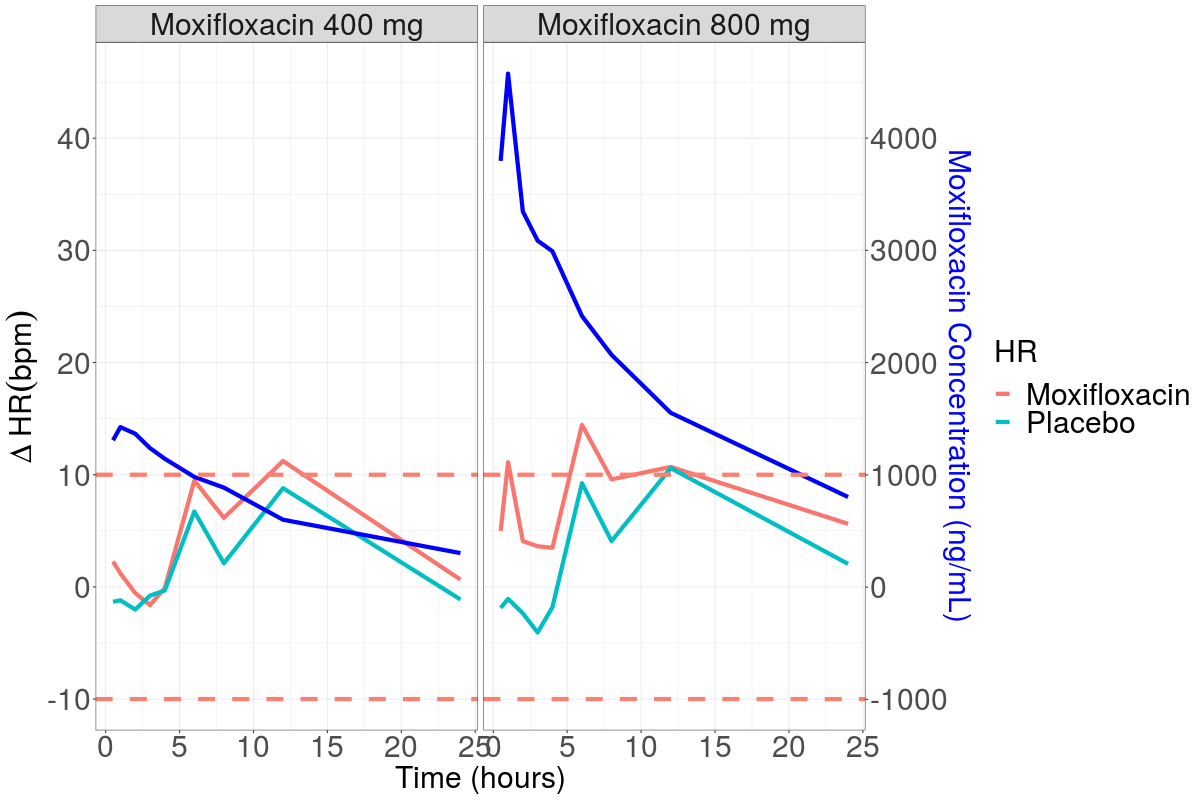
\includegraphics[width=\textwidth]{../Report/Figures/DHR_pk.png}
\label{fig:DHR_pk}
\end{figure}

\begin{figure}[H]
\caption{$\Delta \Delta$HR versus Moxifloxacin Concentration with Model Slope and 90\% Confidence Intervals}
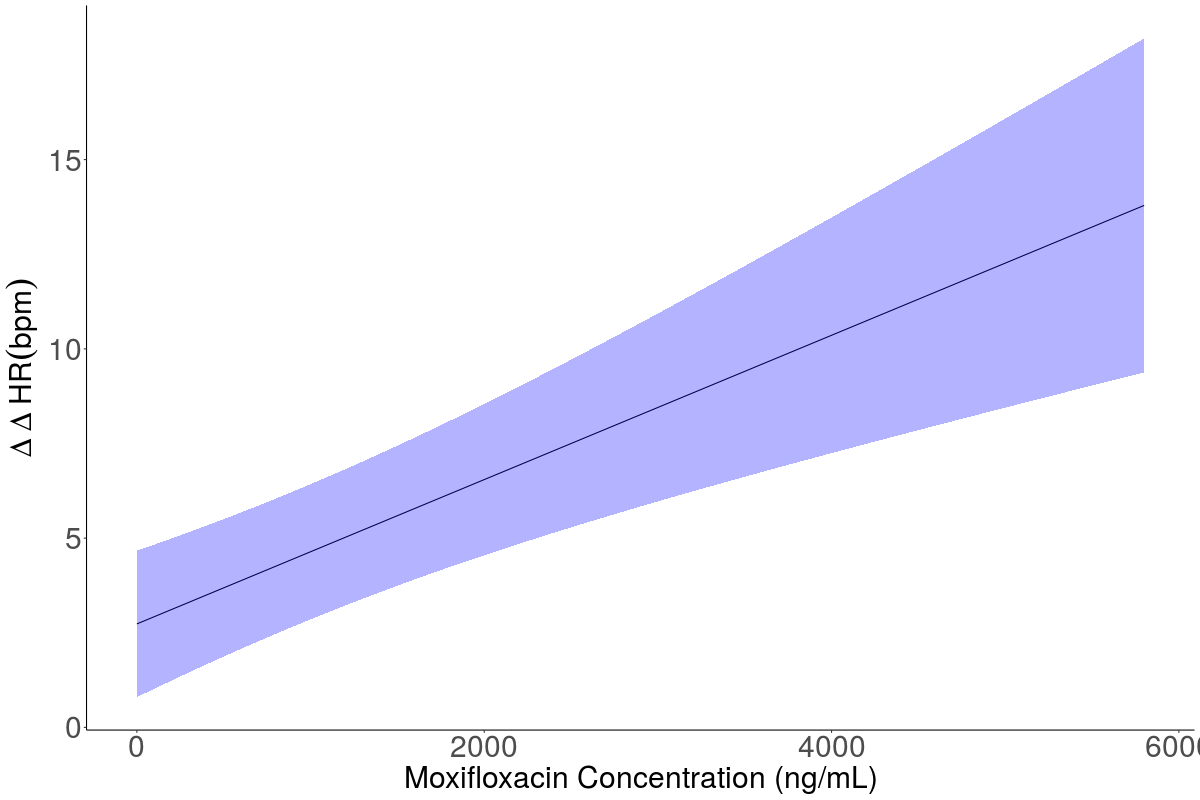
\includegraphics[width=\textwidth]{../Report/Figures/HRvsmoxi.png}
\label{fig:HRvsmoxi}
\end{figure}

\hypertarget{assessment-of-appropriate-qt-correction-factor}{%
\subsection{Assessment of Appropriate QT Correction
Factor}\label{assessment-of-appropriate-qt-correction-factor}}

As Shown in Figure \ref{fig:QTcorrection}, Bazett's method overcorrected
for the trend between the QT and RR intervals (slope estimate of
-0.114), and Fridericia's also did not completely remove the
relationship, with a slope estimate (95\% CI) which was statistically
significantly different from zero (-0.048 {[}-0.057 to -0.038{]}).

\clearpage

\begin{figure}[H]
\caption{Uncorrected and Fixed Correction Factors to Drug-Free QT intervals} 
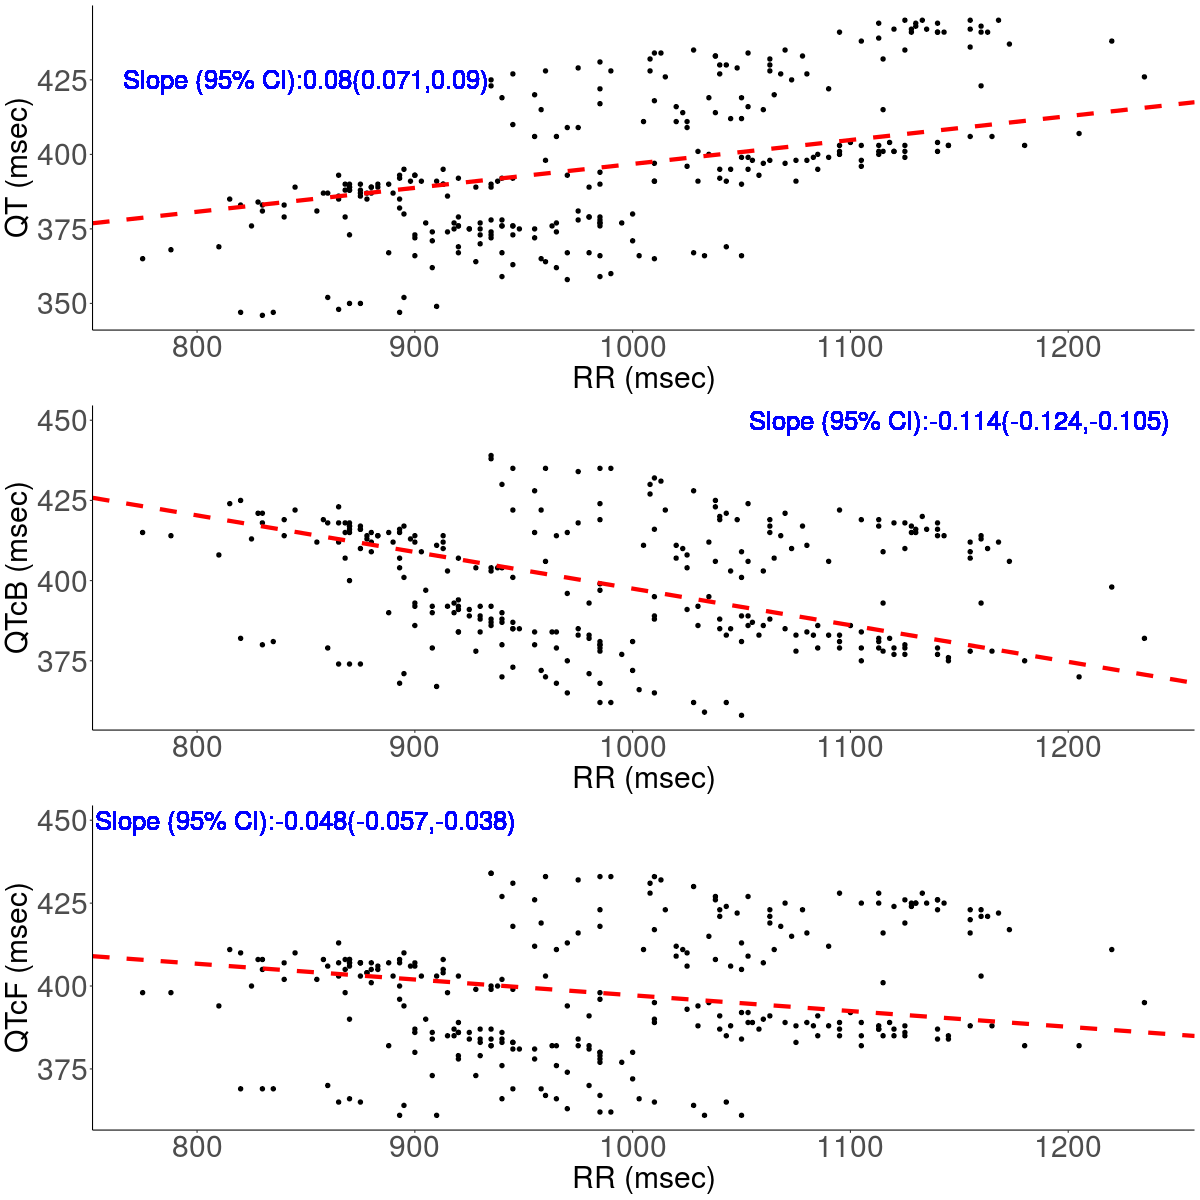
\includegraphics[width=\textwidth]{../Report/Figures/QTcorrection.png}
\label{fig:QTcorrection}
\end{figure}

\hypertarget{assessment-of-time-delay-between-drug-concentration-and-baseline-corrected-qt-intervals}{%
\subsection{Assessment of Time Delay Between Drug Concentration and
Baseline Corrected QT
Intervals}\label{assessment-of-time-delay-between-drug-concentration-and-baseline-corrected-qt-intervals}}

The presence of a delay in the time course of moxifloxacin cardiac
repolarization effect relative to its PK profile was evaluated visually
by plotting and comparing the mean moxifloxacin concentration and
\(\Delta \Delta\)QTcF profiles over time for both moxifloxacin dose
levels (see Figure \ref{fig:DDQTC_pk}). Visual comparison of the mean
moxifloxacin PK and \(\Delta \Delta\)QTcF profiles revealed there was
general concordance in the time course of both PK and cardiac
repolarization, and no time dependency of the \(\Delta \Delta\)QTcF on
moxifloxacin plasma concentration was evident at either dose.

Figure \ref{fig:delta_loess} is a scatter plot of \(\Delta\)QTcF and
drug concentration data with loess smooth line and 95\% confidence
interval and a linear regression line indicating a direct effect between
\(\Delta\)QTc and moxifloxacin concentration.

\begin{figure}[H]
\caption{Overlay of Time course of Mean Moxifloxacin Concentration and Mean $\Delta \Delta$QTcF by Dose} 
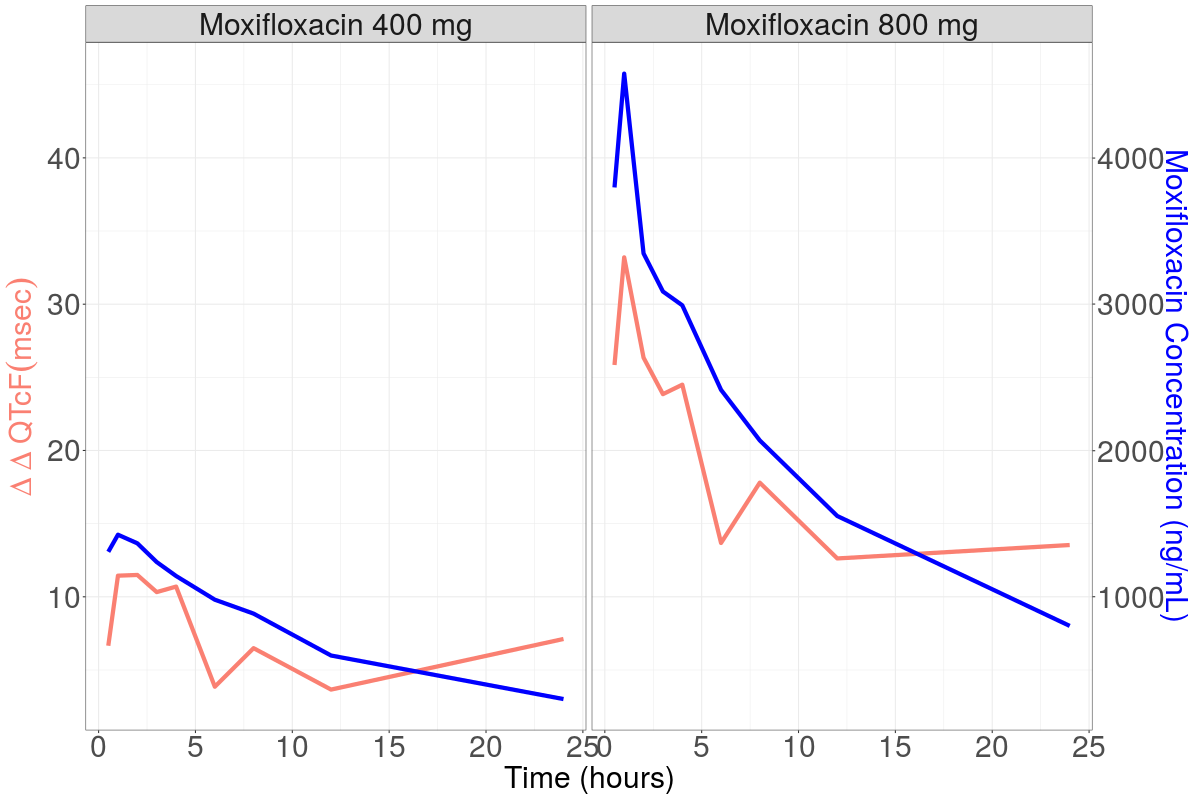
\includegraphics[width=\textwidth]{../Report/Figures/DDQTC_pk.png}
\label{fig:DDQTC_pk}
\end{figure}

\begin{figure}[H]
\caption{Scatter Plot of Paired  Moxifloxacin Concentration and $\Delta$QTcF} 
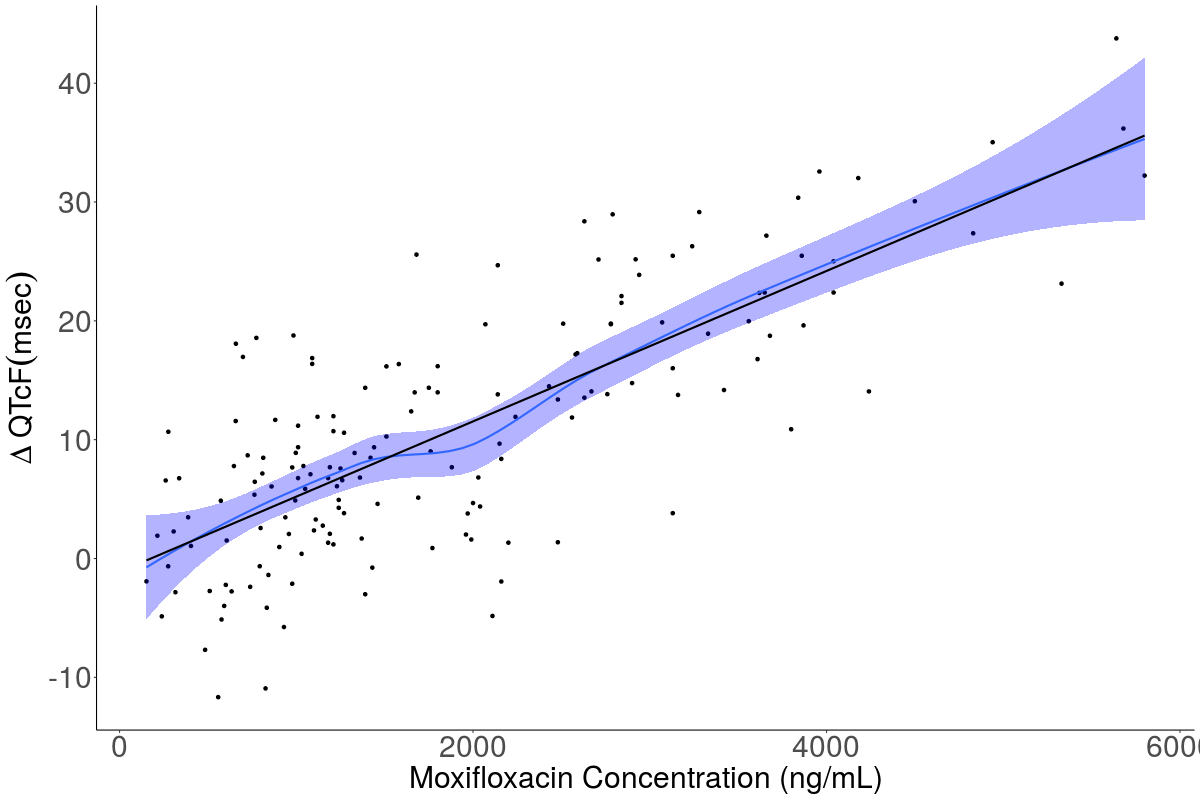
\includegraphics[width=\textwidth]{../Report/Figures/delta_loess.png}
\label{fig:delta_loess}
\end{figure}

\hypertarget{characterization-of-moxifloxacin-exposure-response-relationship-for-qtc-1}{%
\subsection{Characterization of Moxifloxacin Exposure-Response
Relationship for
QTc}\label{characterization-of-moxifloxacin-exposure-response-relationship-for-qtc-1}}

The linear mixed-effects model was fitted to the \(\Delta\)QTcF data for
moxifloxacin and placebo as described in Section \ref{sec:modelfit}. The
results from the model are displayed in Figure \ref{fig:moxifit} and
Table \ref{tab:table.fit}. The mean slope estimated was 0.006
msec/ng/mL, the 90\% confidence interval around the slope estimate
excludes zero indicating positive concentration-dependent effect of
moxifloxacin on \(\Delta\)QTcF intervals. At the therapeutic
moxifloxacin dose of 400 mg, the estimated geometric mean moxifloxacin
Cmax value was calculated to be 1862.1 ng/mL. The estimated mean change
in \(\Delta\)QTcF at the geometric mean Cmax was 15.74 msec with an 90\%
upper bound of 18.43. At the supratherapeutic moxifloxacin dose of 800
mg, the estimated mean change in \(\Delta\)QTcF was 32.1 msec with an
90\% upper bound of 36.21 at the geometric mean Cmax value of 4576.1
ng/mL.

\begin{figure}[H]
\caption{$\Delta \Delta$QTcF versus Moxifloxacin Concentration with Associated Predictions at the Observed Therapeutic and Supratherapeutic Geometric Mean Cmax} 
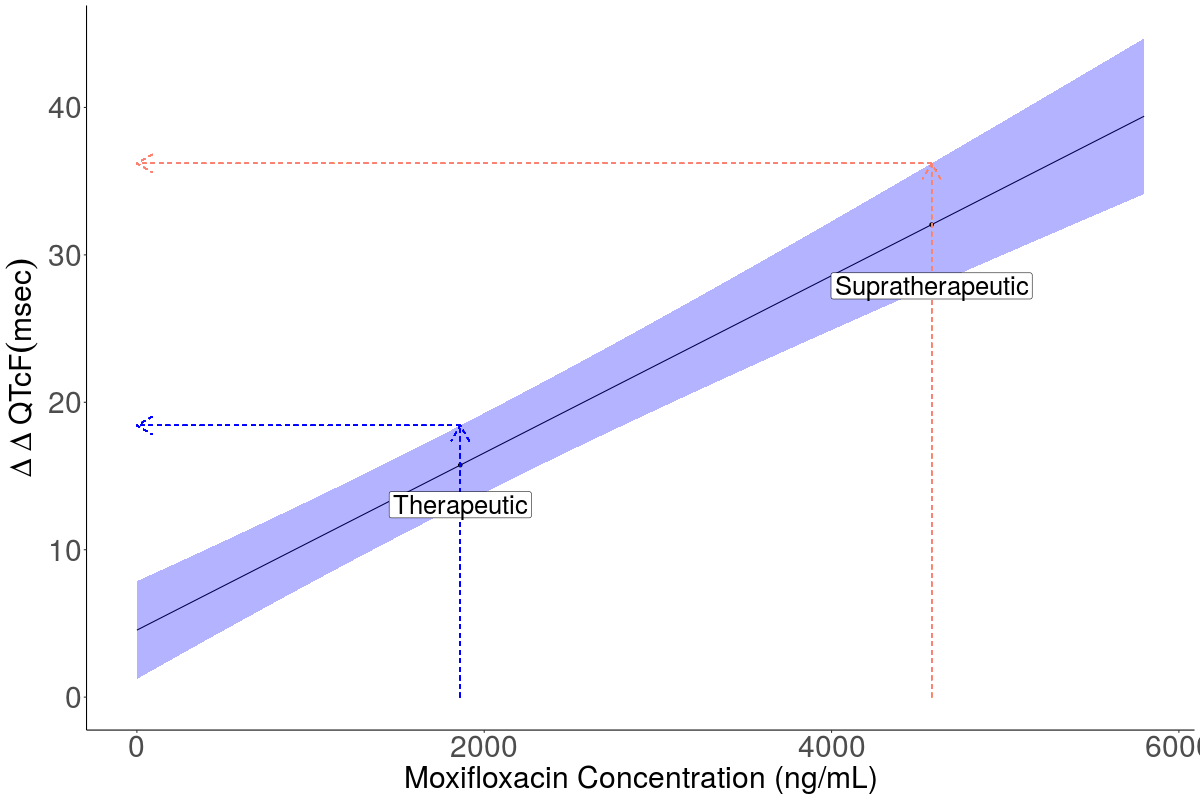
\includegraphics[width=\textwidth]{../Report/Figures/moxifit.png}
\label{fig:moxifit}
\end{figure}

\newpage

\captionsetup{justification = RaggedRight,singlelinecheck=false}
\captionof{table}{Summary of Model Parameter Fit of $\Delta$QTcF Versus Moxifloxacin Concentration}

\begin{tabular}{lrl}
\toprule
Parameter & Estimate & 90\% CI\\
\midrule
TAFDHR 0.5 & -6.676 & (-10.832, -2.519)\\
TAFDHR 1 & -3.433 & (-7.599, 0.734)\\
TAFDHR 12 & -3.644 & (-7.876, 0.588)\\
TAFDHR 2 & -4.743 & (-8.915, -0.571)\\
TAFDHR 24 & -4.130 & (-8.4, 0.141)\\
TAFDHR 24.5 & -4.498 & (-8.862, -0.133)\\
TAFDHR 25 & 0.379 & (-4.155, 4.913)\\
TAFDHR 26 & -4.146 & (-8.429, 0.137)\\
TAFDHR 27 & -4.720 & (-8.967, -0.472)\\
TAFDHR 28 & -5.841 & (-10.076, -1.607)\\
TAFDHR 3 & -4.781 & (-8.959, -0.603)\\
TAFDHR 30 & -6.118 & (-10.302, -1.934)\\
TAFDHR 32 & -8.971 & (-13.138, -4.804)\\
TAFDHR 36 & -2.440 & (-6.605, 1.726)\\
TAFDHR 4 & -5.016 & (-9.199, -0.833)\\
TAFDHR 48 & -4.051 & (-8.262, 0.16)\\
TAFDHR 6 & -2.213 & (-6.408, 1.982)\\
TAFDHR 8 & -6.927 & (-11.13, -2.725)\\
TRTGD - moxifloxacin & 4.547 & (1.23, 7.864)\\
CONC & 0.006 & (0.005, 0.007)\\
DBQTF & -0.055 & (-0.196, 0.085)\\
Random Effects on Intercept & 4.230 & (2.567, 6.97)\\
Cor Intercept-concentration & -0.572 & (-0.991, 0.884)\\
Random Effects on Concentration & 0.001 & (0, 0.003)\\
Residual Error & 5.934 & (5.422, 6.494)\\
\bottomrule
\end{tabular}


\label{tab:table.fit}

\hypertarget{model-adequacy-1}{%
\subsection{Model Adequacy}\label{model-adequacy-1}}

\hypertarget{prediction_based-diagnostics}{%
\subsubsection{Prediction\_based
Diagnostics}\label{prediction_based-diagnostics}}

The scatter plots of model-predicted (population and individual) versus
observed \(\Delta\)QTc values with line of unity and loess line are
presented in Figure \ref{fig:pred_ipred} and do not suggest any patterns
that indicate over or under model-predicted \(\Delta\)QTc.

\begin{figure}[H]
\caption{Population and Individual Model Predictions Diagnostic Plots} 
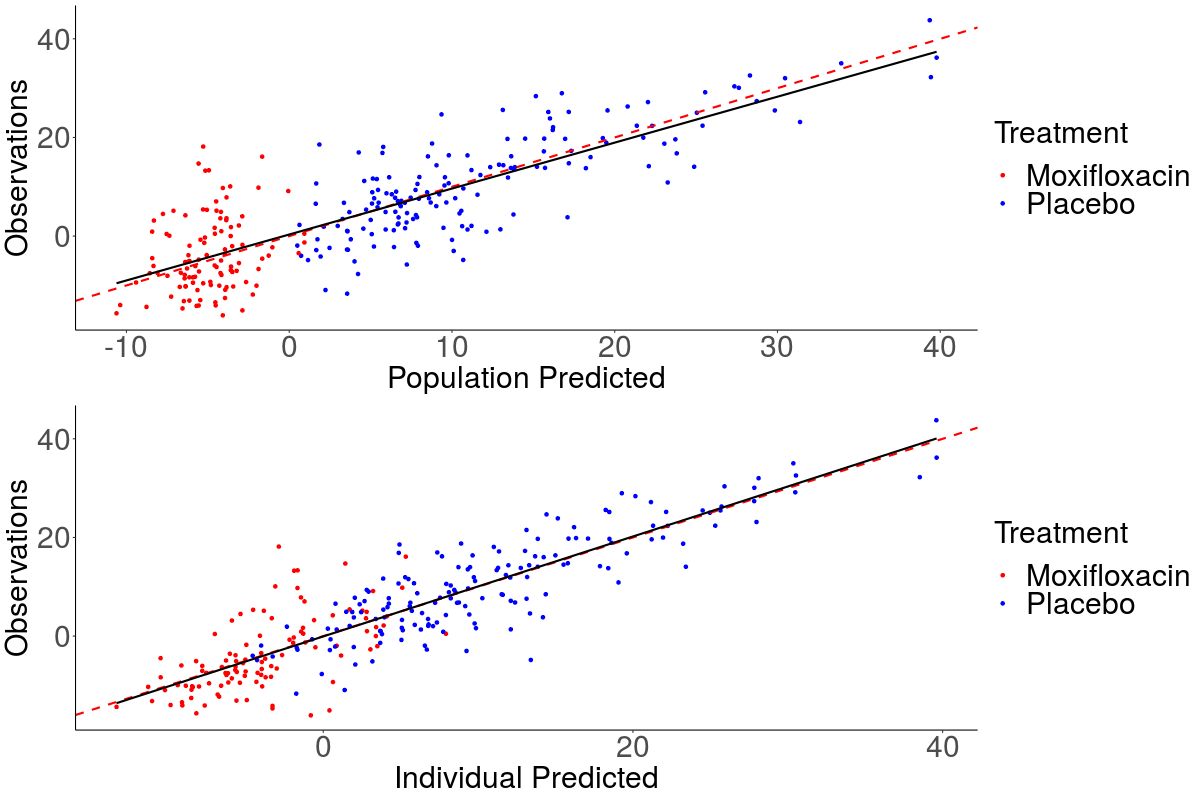
\includegraphics[width=\textwidth]{../Report/Figures/DV_pred_ipred.png}
\label{fig:pred_ipred}
\end{figure}

\hypertarget{residual-based-diagnostics}{%
\subsubsection{Residual-Based
Diagnostics}\label{residual-based-diagnostics}}

Figure \ref{fig:res} presents scatter plots of population and individual
standarized residuals (Pearson weighted) versus population and
individual model predictions of \(\Delta\)QTcF and moxifloxacin plasma
concentrations. In all cases, the residuals are randomly scattered
around zero suggesting lack of model misspecification.

\begin{figure}[H]
\caption{Population and Individual Standardized Residuals versus Population and Individual Model $\Delta$QTc Predictions and Moxifloxacin Concentrations} 
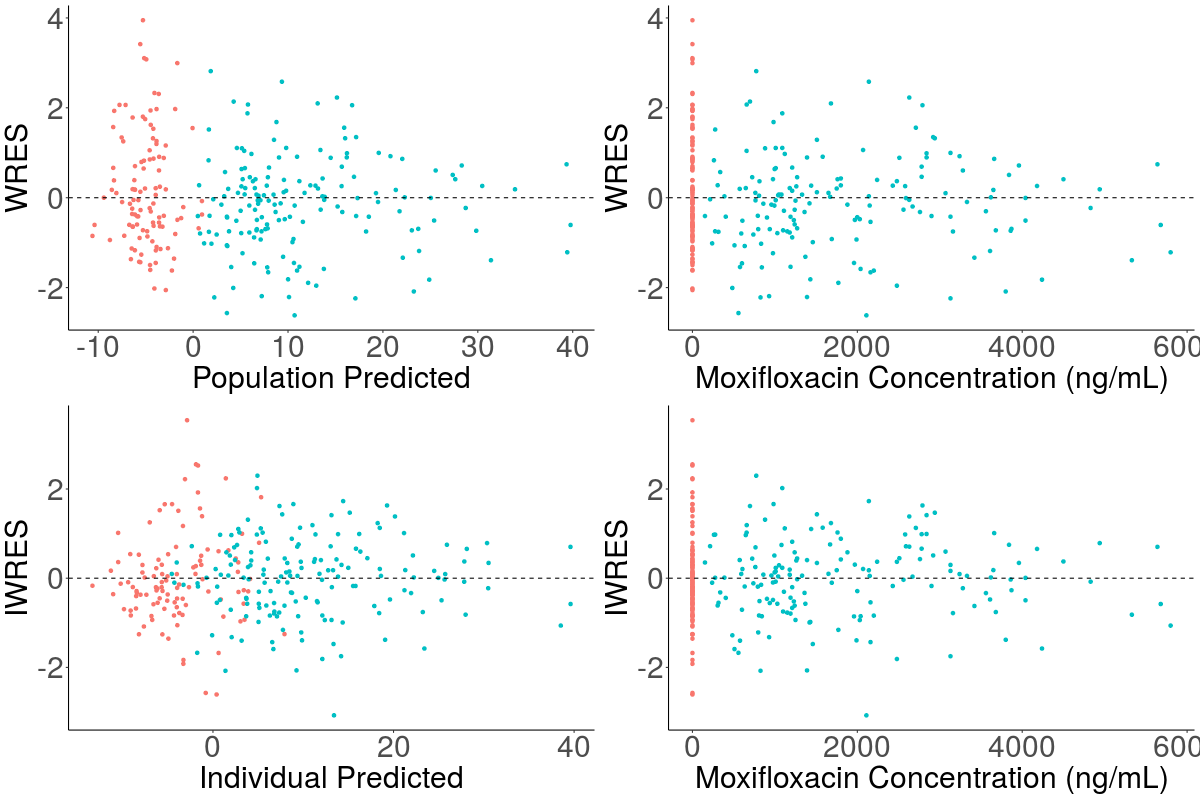
\includegraphics[width=\textwidth]{../Report/Figures/res.png}
\label{fig:res}
\end{figure}

Figure \ref{fig:qq} displays the quantile-quantile plots of residuals.
The residuals fall in the line of unity with no heavy tails indicative
of model misspecification. The residuals follow normal distribution with
a mean of zero.

\begin{figure}[H]
\caption{Quantile-Quantile (Q-Q) Plots of Pearson Weighted Standardized Residuals} 
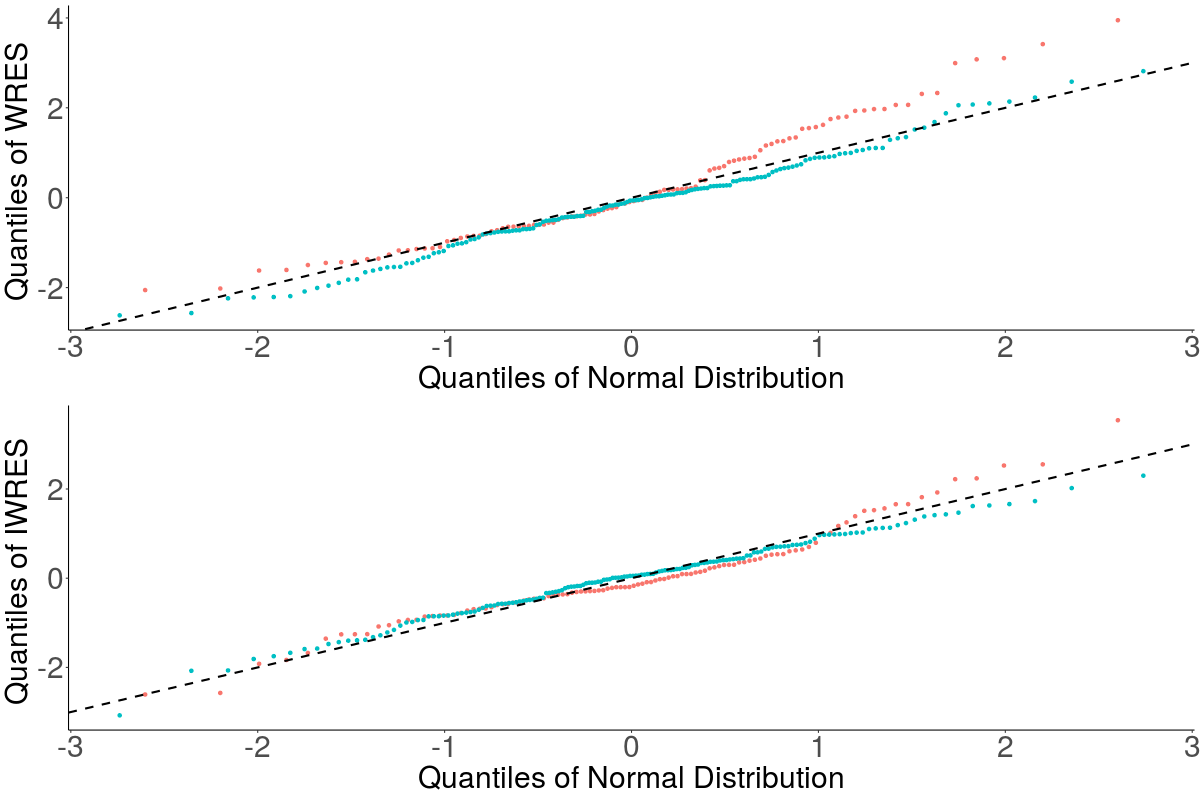
\includegraphics[width=\textwidth]{../Report/Figures/qq.png}
\label{fig:qq}
\end{figure}

Figures \ref{fig:boxplots1} and \ref{fig:boxplots2} are boxplots of
population and individual model residuals versus the nominal timepoints
for the assessments and versus treatment groups, placebo and
moxifloxacin. Residuals are centered around zero not showing any
particular pattern.

\begin{figure}[H]
\caption{Boxplots of Standardized Residuals Versus Nominal Time Postdose} 
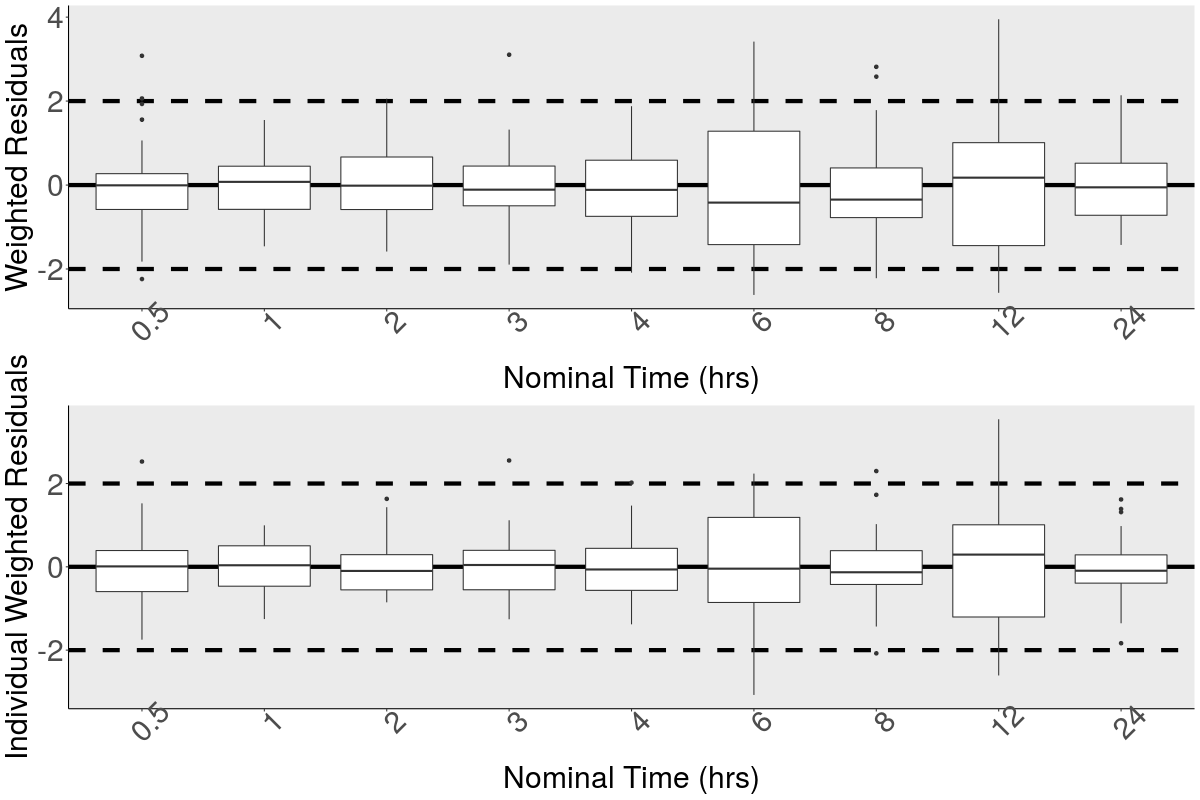
\includegraphics[width=\textwidth]{../Report/Figures/boxplots1.png}
\label{fig:boxplots1}
\end{figure}

\begin{figure}[H]
\caption{Boxplots of Standardized Residuals Versus Treatment} 
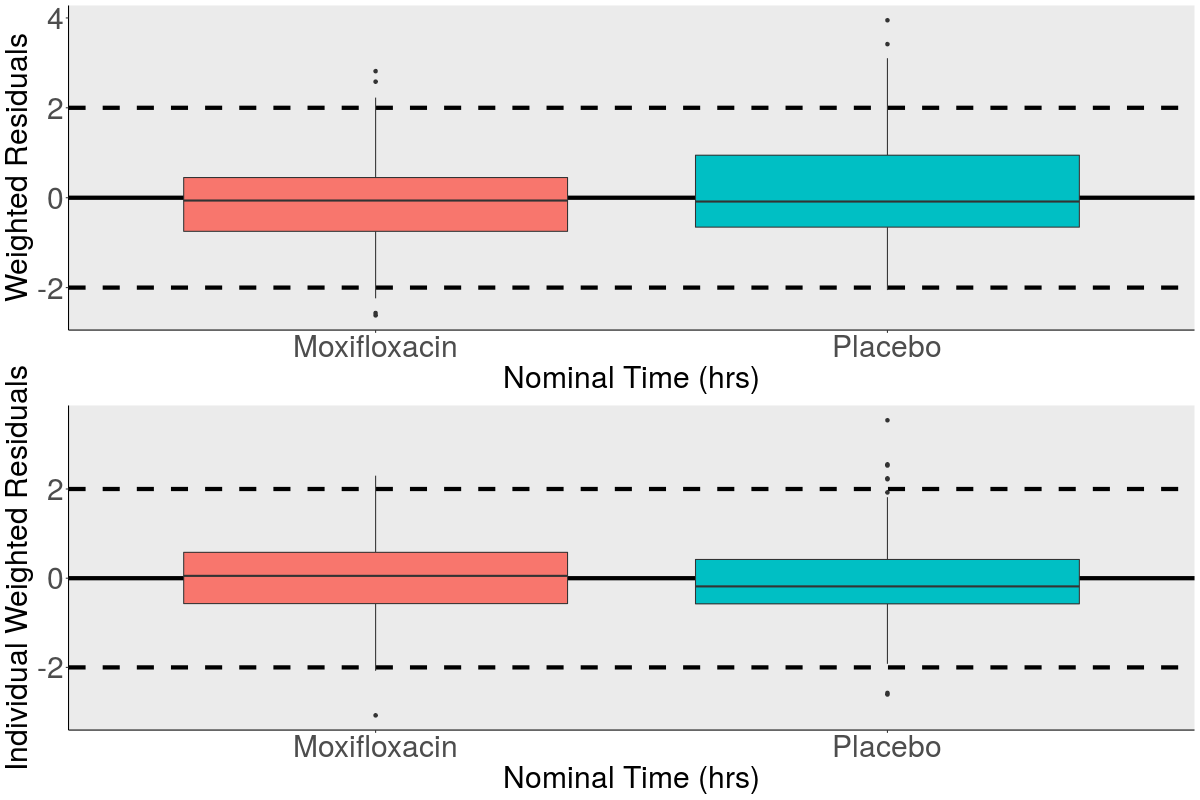
\includegraphics[width=\textwidth]{../Report/Figures/boxplots2.png}
\label{fig:boxplots2}
\end{figure}

\hypertarget{evaluation-of-linear-mixed-effects-model-for-deltaqtc-drug-concentration-relationship}{%
\subsubsection{\texorpdfstring{Evaluation of Linear Mixed-Effects Model
for \(\Delta\)QTc-Drug Concentration
Relationship}{Evaluation of Linear Mixed-Effects Model for \textbackslash DeltaQTc-Drug Concentration Relationship}}\label{evaluation-of-linear-mixed-effects-model-for-deltaqtc-drug-concentration-relationship}}

Figure \ref{fig:DQTCquantile} corresponds to the evaluation of the final
model. Mean baseline-corrected QTcF (\(\Delta\)QTcF) versus moxifloxacin
concentration quantiles derived from the observed data with
model-predicted variables and the associated 90\% CI overlayed.

\begin{figure}[H]
\caption{$\Delta$QTcF versus Moxifloxacin Concentration Quantile Plot} 
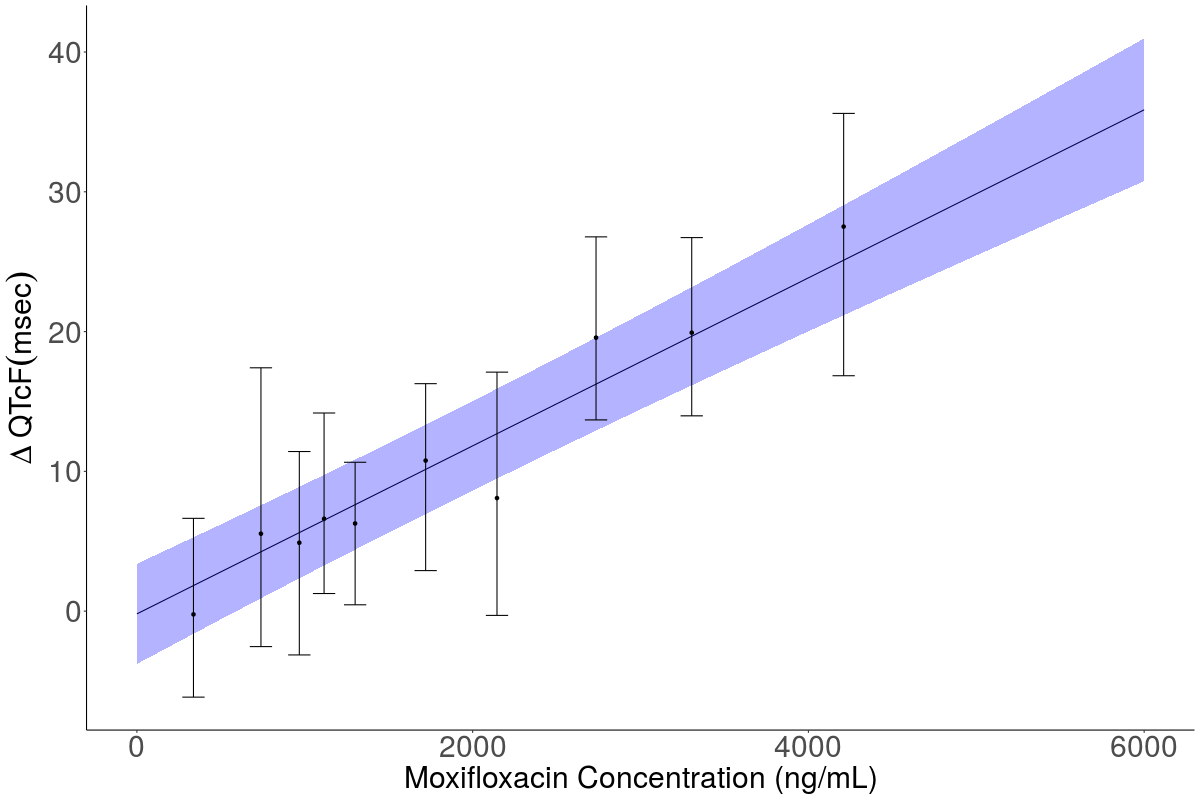
\includegraphics[width=\textwidth]{../Report/Figures/DQTCquantile.png}
\label{fig:DQTCquantile}
\end{figure}

\hypertarget{discussion}{%
\section{Discussion}\label{discussion}}

The ICH
\href{https://database.ich.org/sites/default/files/E14_Q\%26As_R3_Q\%26As.pdf}{E14
Q\&A (R3)} document was revised in December 2015 to confirm
concentration-QTc (C-QT) analyses as an acceptable primary analysis
methodology for definitive QTc characterization. Subsequently, a
\href{https://link-springer-com.eu1.proxy.openathens.net/content/pdf/10.1007/s10928-017-9558-5.pdf}{scientific
white paper on concentration-QTc modeling} was published collaboratively
by regulatory and industry representatives. This paper described the
critical design elements for the studies suitable for such analysis, as
well as modeling and reporting aspects corresponding to regulatory
submissions involving such concentration-QTc analyses. The definitive
C-QT analysis of data in early phase studies following ICH E14 Q\&A (R3)
implementation has alleviated the need for Thorough QT/QTc (TQT) studies
for multiple development programs. In this example report we used
moxifloxacin data from the
\href{https://pubmed.ncbi.nlm.nih.gov/25670536/}{IQ-CSRC study} .

The results of the analysis for the moxifloxacin IQ-CSRC study indicated
the presence of the expected effect of moxifloxacin on the QTcF interval
at the therapeutic and supratherapeutic doses, as the upper bound of the
2-sided 90\% CIs was above the pre-specified criterion of 10 msec.

\hypertarget{conclusions}{%
\section{Conclusions}\label{conclusions}}

This analysis represents the quantitative evaluation of the relationship
between changes in the placebo-adjusted change from baseline QTc
interval and plasma concentrations of moxifloxacin.

\begin{itemize}
\item
  Moxifloxacin does not have a meaningful effect on heart rate (change
  in the RR interval); the fixed corrections (QTcF) utilized in this
  analysis was considered sufficient to correct for the underlying
  relationship between RR and QT intervals.
\item
  The final QTc\_Concentration model for \(\Delta\)QTcF indicated a mean
  estimate of a 0.006 msec increase from baseline in QTcF per ng/mL of
  moxifloxacin. At the geometric mean therapeutic Cmax value observed in
  patients (400 mg dose), the mean predicted increase in
  placebo-adjusted change from baseline QTcF is 15.74 msec, and the
  upper bound of the 90\% CI of \(\Delta \Delta\)QTcF is above 10 msec
  (18.43).
\item
  At the geometric mean supratherapeutic moxifloxacin Cmax value
  observed in patients (800 mg dose), the mean predicted increase in
  placebo-adjusted change from baseline QTcF is 32.05 msec and the upper
  bound of the 90\% CI of \(\Delta \Delta\)QTcF is above the 10 msec
  threshold (36.21).
\end{itemize}

\clearpage

\renewcommand\refname{References}
  \bibliography{references.bib}

\end{document}
